%%%%%%%%%%%%%%%%%%%%%%%%%%%%%%%%%%%%%%%%%
% Beamer Presentation
% LaTeX Template
% Version 1.0 (10/11/12)
%
% This template has been downloaded from:
% http://www.LaTeXTemplates.com
%
% License:
% CC BY-NC-SA 3.0 (http://creativecommons.org/licenses/by-nc-sa/3.0/)
%
%%%%%%%%%%%%%%%%%%%%%%%%%%%%%%%%%%%%%%%%%

%----------------------------------------------------------------------------------------
%	PACKAGES AND THEMES
%----------------------------------------------------------------------------------------

\documentclass{beamer}

\mode<presentation> {

% The Beamer class comes with a number of default slide themes
% which change the colors and layouts of slides. Below this is a list
% of all the themes, uncomment each in turn to see what they look like.

%\usetheme{default}
%\usetheme{AnnArbor}
%\usetheme{Antibes}
%\usetheme{Bergen}
%\usetheme{Berkeley}
%\usetheme{Berlin}
%\usetheme{Boadilla}
%\usetheme{CambridgeUS}
%\usetheme{Copenhagen}
%\usetheme{Darmstadt}
%\usetheme{Dresden}
%\usetheme{Frankfurt}
%\usetheme{Goettingen}
%\usetheme{Hannover}
%\usetheme{Ilmenau}
%\usetheme{JuanLesPins}
%\usetheme{Luebeck}
%\usetheme{Madrid}
%\usetheme{Malmoe}
%\usetheme{Marburg}
%\usetheme{Montpellier}
%\usetheme{PaloAlto}
%\usetheme{Pittsburgh}
%\usetheme{Rochester}
%\usetheme{Singapore}
%\usetheme{Szeged}
\usetheme{Warsaw}

% As well as themes, the Beamer class has a number of color themes
% for any slide theme. Uncomment each of these in turn to see how it
% changes the colors of your current slide theme.

%\usecolortheme{albatross}
%\usecolortheme{beaver}
%\usecolortheme{beetle}
%\usecolortheme{crane}
%\usecolortheme{dolphin}
%\usecolortheme{dove}
%\usecolortheme{fly}
%\usecolortheme{lily}
%\usecolortheme{orchid}
%\usecolortheme{rose}
%\usecolortheme{seagull}
%\usecolortheme{seahorse}
%\usecolortheme{whale}
%\usecolortheme{wolverine}

%\setbeamertemplate{footline} % To remove the footer line in all slides uncomment this line
%\setbeamertemplate{footline}[page number] % To replace the footer line in all slides with a simple slide count uncomment this line

%\setbeamertemplate{navigation symbols}{} % To remove the navigation symbols from the bottom of all slides uncomment this line
}

\usepackage{graphicx} % Allows including images
\usepackage{booktabs} % Allows the use of \toprule, \midrule and \bottomrule in tables

%----------------------------------------------------------------------------------------
%	TITLE PAGE
%----------------------------------------------------------------------------------------

\title[NS Structure and Evolution]{The Equations of Stellar Structure and Evolution in Neutron Stars} % The short title appears at the bottom of every slide, the full title is only on the title page

\author{Kraig Andrews} % Your name
\institute[Michigan State Univeristy] % Your institution as it will appear on the bottom of every slide, may be shorthand to save space
{
Michigan State University \\ % Your institution for the title page
\medskip
\textit{andre220@msu.edu} % Your email address
}
\date{\today} % Date, can be changed to a custom date

\begin{document}

\begin{frame}
\titlepage % Print the title page as the first slide
\end{frame}

\begin{frame}
\frametitle{Overview} % Table of contents slide, comment this block out to remove it
\tableofcontents % Throughout your presentation, if you choose to use \section{} and \subsection{} commands, these will automatically be printed on this slide as an overview of your presentation
\end{frame}

%----------------------------------------------------------------------------------------
%	PRESENTATION SLIDES
%----------------------------------------------------------------------------------------


%------------------------------------------------
\section{The Equations of Stellar Structure and Evolution} % Sections can be created in order to organize your presentation into discrete blocks, all sections and subsections are automatically printed in the table of contents as an overview of the talk
%-----------------------------------------------

\subsection{Non-Relativistic Regime: Newtownian Mechanics} % A subsection can be created just before a set of slides with a common theme to further break down your presentation into chunks

\subsection{Neutron Stars}
\subsection{Relativistic Regime: The TOV Equations}

\section{The Equation of State}
\subsection{Polytrope}
\subsection{Equation of State within Neutron Stars}

\section{Solving the TOV Equations}
\subsection{Numerical Methods}
\subsection{Code Structure}

\section{Results}
\subsection{Mass Radius Curves}
%-----------------------------------------------
\begin{frame}
\frametitle{Motivation}
Why study neutron stars?
\begin{itemize}
\item The equations of stellar structure and evolution connect an equation of state (EOS) to set of mass and radius points
\item Can take observed data of mass and radius and obtain an EOS
\item Can use an experimental EOS to produce a family of mass-radius data
\end{itemize}
\end{frame}
%-----------------------------------------------
\begin{frame}
\frametitle{Equations of Stellar Structure: Newtonian Picture}
Determine the equations of stellar structure and evolution for single star without any significant contributing forces other than pressure and gravity acting upon the mass element.
\begin{equation}\label{eq:pda}
P(r) dA - [P(r) + dP]dA - \rho(r) dA dr g(r) = 0
\end{equation}
\begin{itemize} 
\item Assume hydrostatic equilibrium within the star
\end{itemize}
\begin{equation}\label{eq:hydro}
\frac{dP(r)}{dr} = -\rho(r) g(r)
\end{equation}
\begin{itemize}
\item This implies that the pressure, $P$ increases as the radial coordinate decreases.
\end{itemize}
\end{frame}

\begin{frame}
\frametitle{Equations of Stellar Structure: Newtonian Picture}
The Newtonian equations for stellar structure assuming hydrostatic equilibrium:
\begin{equation}\label{eq:dpdr}
\frac{dP(r)}{dr} = -\frac{GM\rho}{r^2}
\end{equation}
\begin{equation}\label{eq:dmdr}
\frac{dM(r)}{dr} = 4\pi r^2 \rho
\end{equation}
\begin{itemize}
\item To fully solve eqs.~(\ref{eq:dpdr},~\ref{eq:dmdr}) for any point in the star an equation of state (EOS) is needed.
\end{itemize}
\end{frame}

%------------------------------------------------

\begin{frame}
\frametitle{Equations of Stellar Structure: Neutron Stars}
\begin{itemize}
\item Moving to more complex stellar structures eqs.~(\ref{eq:dpdr},~\ref{eq:dmdr}) need to be altered.
\item The Newtonian gravitational theory is no longer valid for the case of neutron stars. 
\item Neutron stars are compact objects and General Relativitistic theory takes over.
\end{itemize}
\end{frame}

%------------------------------------------------

\begin{frame}
\frametitle{Equations of Stellar Structure: Neutron Stars}
\begin{itemize}
\item The idea of compact stars consisting of dense atomic nuclei was proposed by Landau in 1932, before the discovery of the neutron \cite{landau}.
\item Shortly after the discovery of the neutron, the prediction of such stars was confirmed while seeking an explanation for the origin of supernovae \cite{baade}.
\item The first models of neutron stars emerged in 1939 formulated by Tolman Oppenheimer and Volkoff, and would become known as the TOV equations \cite{tov1939}.
\end{itemize}

\end{frame}

%------------------------------------------------
\begin{frame}
\frametitle{Equations of Stellar Structure: General Relativistic Picture}
Eqs.~(\ref{eq:dmdr},~\ref{eq:dpdr}) must be altered for the case of neutron stars. 
\begin{itemize}
\item We begin with the Einstein equation
\begin{equation}\label{eq:einstein}
G^{\mu\nu} = 8\pi T^{\mu\nu},
\end{equation}
where $G^{\mu\nu}$ is the Einstein tensor and $T^{\mu\nu}$ is the stress energy tensor. 
\end{itemize}

We make the following assumptions
\begin{itemize}
\item Spherical Symmetry
\item Perfect fluid
\item Non-rotating body in hydrostatic equilibrium
\end{itemize} 
\end{frame}

%------------------------------------------------

%\begin{frame}
%\frametitle{Equations of Stellar Structure: General Relativistic Picture}
%\begin{itemize}
%\item Spherical Symmetry: the line element \\
%\begin{equation}\label{eq:line}
%ds^2 = -e^{\sigma(r)}dt^2 + e^{\lambda(r)} dr^2 + r^2 d\theta^2 + r^2 sin^2\theta d\phi^2
%\end{equation}
%\item Perfect fluid: the stress tensor becomes \\
%\begin{equation}\label{eq:stress}
%T^\mu_\nu = (\epsilon + P)u^\mu u_\nu - P \delta^\mu_\nu
%\end{equation}
%\item Non-rotating body in hydrostatic equilibrium
%\end{itemize}
%\end{frame}
%-------------------------------------------------------
\begin{frame}
\frametitle{Equations of Stellar Structure: General Relativistic Picture}
Using the above information and employing known constaints on the Einstein tensors we arrive at the following equations
\begin{equation}\label{eq:dp-tov}
\frac{dP(r)}{dr} = -\frac{Gm\epsilon}{r^2}(1 + \frac{P}{\epsilon c^2})(1+\frac{4\pi r^3 P}{mc^2})(1-\frac{2Gm}{rc^2})^{-1}.
\end{equation}
\begin{equation}\label{eq:dm-tov}
\frac{dM(r)}{dr} = 4\pi \epsilon r^2,
\end{equation}
These are known the equations known as the TOV equations \cite{tov1939}.
\end{frame}
%------------------------------------------------------
\begin{frame}
\frametitle{Solving the TOV Equations: Numerical Methods}
To solve the differential eqs.~(\ref{eq:dm-tov},~\ref{eq:dp-tov}) we will use the method of Runge Kutta integration. \\

To do this we combine several Euler-like steps assuming that we are given the IVP 
\begin{equation}\label{eq:dxdy}
\frac{dx}{dy} = f(x,y),
\end{equation}
with initial values $y = y_0$ at $x = x_0$. Then the differential equation can be solved numerical expanded Euler steps, with some step-size $\delta x$.
\end{frame}
%----------------------------------------------------------
\begin{frame}
\frametitle{Solving the TOV Equations: Numerical Methods}
To perform one step in the integration of eq.~(\ref{eq:dxdy}) the following are calculated
\begin{eqnarray}
&& k_1 = \delta x f(x_0,y_0), \\
&& k_2 = \delta x f(x_0 + 0.5\delta x, y_0 + 0.5 k_1), \\
&& k_3 = \delta x f(x_0 + 0.5 \delta x, y_0 + 0.5 k_2), \\
&& k_4 = \delta x f(x_0 + \delta x, y_0 + k_3).
\end{eqnarray}
Thus the next step $x_{n+1}$ is given by
\begin{equation}
x_{n+1} = x_n + \frac{1}{6}(k_1 + 2k_2 + 2k_3 + k_4)
\end{equation}
\end{frame}
%------------------------------------------------
%\section{The Equation of State}
%------------------------------------------------
\begin{frame}
\frametitle{The Equation of State: Polytrope}
To solve the equations of stellar structure for either the Newtonian or relativistic case we need a relationship between the pressure and density at points within the star.

The interior of a neutron star has varying densities in different regions. 

\begin{itemize}
\item Core:\\
In the core throughout computation a polytrope is used 
\begin{equation}\label{eq:eos_core}
P = K \epsilon^\gamma
\end{equation}
\item Crust: \\
In the crust an interpolation function was used with data from Steiner et. al
\begin{equation}\label{eq:interp}
\rho = \rho_1 + \frac{\rho_2 - \rho_1}{P_2 - P_1}(P - P_1)
\end{equation}
\end{itemize}
\end{frame}
%-------------------------------------------------------
\begin{frame}
\frametitle{Solving the TOV Equations: Code Structure}
Solving eqs.~(\ref{eq:dm-tov},~\ref{eq:dp-tov}) to obtain a mass-radius curve

Boundary Conditions:
\begin{itemize}
\item $M(r = 0) = 0$
\item $\epsilon(r = 0) = \epsilon_c$
\item $P(r = 0) = P_c$
\end{itemize}
\end{frame}
%-------------------------------------------------------
\begin{frame}
\frametitle{Solving the TOV Equations: Code Structure}
Algorithm for solving the TOV equations numerically
\begin{itemize}
\item Using Runge Kutta advance one steps: $M_{i+1}$ and $P_{i+1}$
\item From $P_{i+1}$ use defined EOS to get $\epsilon_{i+1}$
\item These values are the initial points for the next iteration
\item If $P_{k+1} \le P_{stop}$ then stop \\
$\implies$ $M_k = M(r_k) = M$ and $r_k = R$
\end{itemize}
\end{frame}
%-------------------------------------------------------
\begin{frame}
\frametitle{Solving the TOV Equations: Results}
\begin{figure}
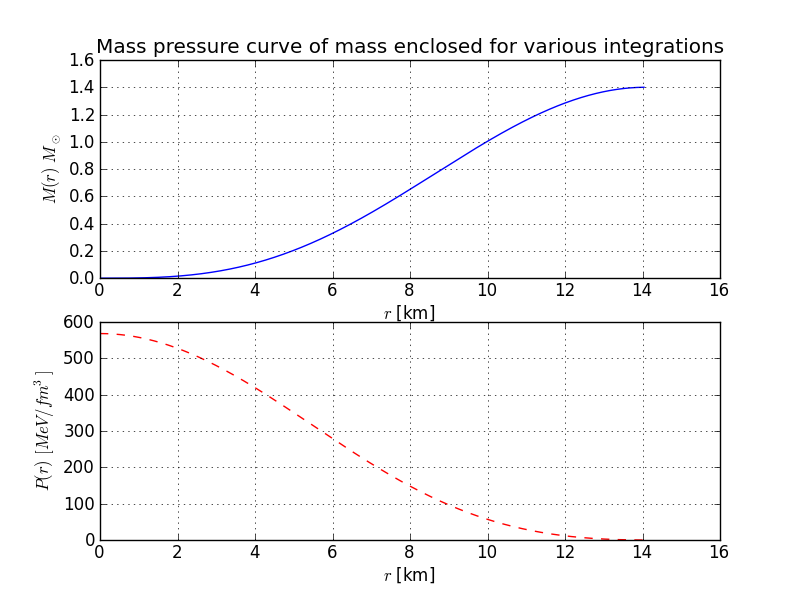
\includegraphics[width=0.6\linewidth]{figs/14mass.png}
\caption{Mass enclosed curve for a $1.4 M_\odot$ mass neutron star with a total radius of $14$ $\textrm{km}$. Obtained for one integration of the TOV equations.}
\end{figure}
\end{frame}
%-------------------------------------------------------
\begin{frame}
\frametitle{Solving the TOV Equations: Results}
\begin{figure}
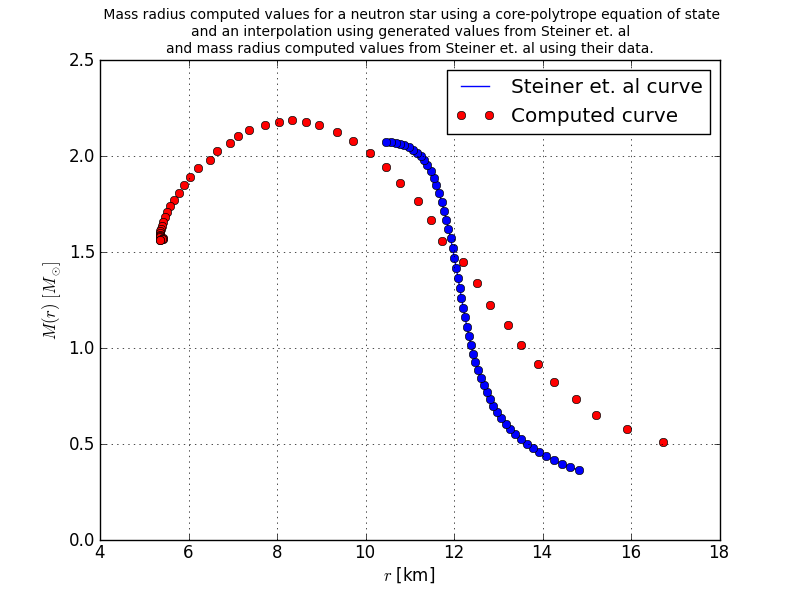
\includegraphics[width=0.6\linewidth]{figs/mestein.png}
\caption{Mass-radius curve for computed solutions to TOV eqs. and Steiner et. al data values \cite{steiner2010}.}
\end{figure}
\end{frame}
%------------------------------------------------------
\begin{frame}
\frametitle{Conclusions: Future Considerations}
For future work the following ideas would be implemented
\begin{itemize}
\item Implement a more realistic EOS in the core (dependent on baryon number, nuclear interactions, etc...)
\item Use Monte Carlo methods to obtain constraints on the EOS based on MCMC fit results
\end{itemize}
\end{frame}
%-------------------------------------------------------
\begin{frame}
\frametitle{References}
\footnotesize{
\begin{thebibliography}{99} % Beamer does not support BibTeX so references must be inserted manually as below
\bibitem[Landau, 1932]{landau} L.D. Landau (1932)
\newblock On the Theory of Stars
\newblock \emph{Phys. Z. Sowjetunion} (1).

\bibitem[Baade, 1934]{baade} W. Baade \& F. Zwicky (1934)
\newblock Supernovae and Cosmic Rays
\newblock \emph{Phys. Rev.} (45) 138.

\bibitem[Oppenheimer, 1939]{tov1939} Oppenheimer, J.R. and Volkoff, G.M. \& Tolman, R.C. (1939)
\newblock On Massive Neutron Cores
\newblock \emph{Phys. Rev.} (55) 374-381.

\bibitem[Steiner et. al, 2010]{steiner2010} Steiner, A.W, Lattimer, J.M and Brown, E.F. (2010)
\newblock The Equation of State from Observed Masses and Radii of Neutron Stars
\newblock \emph{ApJ} 33-54.

\end{thebibliography}
}

\end{frame}

%------------------------------------------------

\begin{frame}
\Huge{\centerline{The End}}
\end{frame}

%----------------------------------------------------------------------------------------

\end{document} 
